\documentclass{tktltiki}
\usepackage{url}
\begin{document}
\title{Keskitetty tunnistautuminen Ruby on Rails -ohjelmistokehyksessä}
\author{Olli Jokinen}
\date{\today}
\level{Pro gradu -tutkielma}
\maketitle
\doublespacing
\faculty{Matemaattis-luonnontieteellinen}
\department{Tietojenkäsittelytieteen laitos}
\subject{Tietojenkäsittelytiede}
\depositeplace{Tietojenkäsittelytieteen laitoksen kirjasto}
\additionalinformation{}
\numberofpagesinformation{\numberofpages\ sivua +
\numberofappendixpages[100] liitesivua}
\classification{A.1 [Introductory and Survey] \\
I.7.m [Document and Text Processing]: Miscellaneous}
\keywords{avainsana}
\begin{abstract}
Tutkielmassa selvitetään keskitetyn tunnistautumispalvelun toteuttamista palveluperustaisten arkkitehtuurien mukaisissa web-sovellusympäristöissä. Painopisteenä ovat sovellusympäristöt, joissa ollaan siirtymässä palveluperustaisiin arkkitehtuureihin. Tutkielmassa käytetään esimerkkinä tällaisesta ympäristöstä Kapsi Internet-käyttäjät ry:n jäsenhallintatyökaluja, joiden tunnistautuminen muutetaan keskitetyn tunnistautumispalvelun tehtäväksi.

Ensimmäiseksi tutkielmassa esitellään web-sovellusten kehitys varhaisista CGI-ohjelmista kohti palveluperustaisten arkkitehtuurien mukaisia web-sovelluksia ja esitellään tunnistautumisen tarpeet tällaisissa arkkitehtuureissa sekä käydään läpi turvallisuuden osatekijöitä ja tavallisia tunnistautumiseen liittyviä ongelmia web-sovelluksissa. Seuraavaksi hahmotellaan tunnistautumisongelman ratkaisuun tarkoitettu keskitetty tunnistautumispalvelu sekä pohditaan sen etuja ja haittoja verrattuna nykyisin yleisesti käytettyihin tunnistautumismekanismeihin.

Sitten tutkitaan tunnistautumispalvelun ja web-sovelluksen väliseen rajapintaan käytettäviä protokollia (SAML, OpenID ja OAuth) ja esitellään OAuth-protokollaa käyttävä Kapsin web-sovellusarkkitehtuuri. Esitetyn arkkitehtuurin etuja ja haittoja sekä sen soveltamista muihin vastaaviin ympäristöihin tutkitaan myös. Arkkitehtuurin laajentamista keskitettyyn pääsynvalvontaan ja kertakirjautumiseen pohditaan tutkielman loppupuolella. Lopuksi pohditaan ulkoisen tunnistautumispalvelun käyttöä, esimerkkinä käytetään Facebookin tarjoamaa tunnistautumisrajapintaa.
\end{abstract}
\mytableofcontents
\section{Johdanto}
Tunnistautumiseen liittyvien käsitteiden läpikäynti ennen protokollien yksityiskohtaista esittelyä auttaa tunnistautumiseen liittyvien periaatteiden hahmottamista. Käsitteet ovat yleisluontoisia ja eivätkä kosketa vain tiettyjä protokollaa. Protokollien yhteydessä käytetään käsitteitä asiakasohjelma, tunnistautumispalvelu, suojattu resurssi, valtuutustieto (credentials), valtuutusavain (authorization code) ja pääsyvaltuutus (access token) \cite{nisti}.

Asiakasohjelmalla tarkoitetaan web-palvelun käyttäjän pääteohjelmaa, jolla hän kirjautuu web-palveluun käyttäen keskitettyä tunnistautumispalvelua. Käytännössä asiakasohjelma on web-palvelun tapauksessa käyttäjän WWW-selain, joka pystyy tekemään uudelleenohjauksia sivustolta toiselle. Uudelleenohjaus on HTTP-protokollan perustoiminnallisuutta, joten mikä tahansa HTTP/1.1-standardin WWW-selain käy asiakasohjelmaksi \cite{rfc2616}.

Tunnistautumispalvelu on web-palvelu, johon käyttäjä ohjataan tekemään tunnistautuminen. Onnistuneen tunnistautumisen jälkeen tunnistautumispalvelu ohjaa asi\-a\-kas\-oh\-jel\-man takaisin tunnistautumista pyytäneen palvelun määrittelemään osoitteeseen \cite{nisti}. Avoimen Internetin puolella tunnistautumispalvelu voi olla esimerkiksi Facebook tai LinkedIn.

Tunnistautumisprotokollien yhteydessä suojatulla resurssilla tarkoitetaan resurssia, jonka käyttö vaatii tunnistautumisen ja käyttöoikeuden. Yleisessä tapauksessa suojatulla resurssilla tarkoitetaan yksittäistä resurssia (käyttäjän valokuvaa), johon halutaan asettaa pääsyrajoituksia \cite{nisti}. Tämän tutkielman puitteissa suojatulla resurssilla tarkoitetaan tunnistautumista vaativaa web-palvelua.

Valtuutustieto koostuu yksilöivästä tunnisteesta ja siihen liittyvästä salaisesta avaimesta. Tämän tutkielman puitteissa valtuutustiedolla tarkoitetaan käyttäjän tunnusta ja salasanaa.

Kirjauduttuaan sisään tunnistautumispalvelimelle, käyttäjä saa valtuutusavaimen, jonka hän lähettää eteenpäin suojatun resurssin omistajalle. Valtuutusavain ei pidä sisällään käyttäjän valtuutustietoja, vaan ainoastaan tunnistautumispalvelin osaa lukea sen \cite{nisti}. Saatuaan valtuutusavaimen käyttäjältä voi suojatun resurssin omistaja hakea pääsyvaltuuden käyttäjän tietoihin tunnistautumispalvelusta.

Pääsyvaltuutus on tunnistautumispalvelimelta saatava yksilöivä tunniste, jonka avulla suojatun resurssin omistaja voi pyytää käyttäjän tiedot tunnistautumispalvelulta. Pääsyvaltuutus on voimassa tietyn ajan, jonka jälkeen se täytyy uusia tunnistautumispalvelimella \cite{nisti}. Pääsyvaltuutusta voidaan käyttää myös tunnistautumispalvelusta erillään olevien resurssien valtuuttamiseen. Esimerkiksi web-sovellus voi hakea tunnistautumispalvelulta pääsyvaltuuden, jolla hän hakee valokuvia valokuvien jakopalvelusta \cite{facebook}.
\section{Ongelmakenttä}
\section{Teknologiat}
\subsection{LDAP}
\subsection{OAuth}
Tämä kappale tulee luultavasti muuttumaan, yleisiä juttuja johdantoon ja tähän vain Oauth-spesifistä asiaa, miten eroaa kerberoksesta jne. Pituus 2-3 sivua, kuvia yms. Oleellisin näistä protokollista, koska tullaan käyttämään toteutuksessa.

OAuth on avoin tunnistautumisrajapinta hajautetuille web-sovelluksille. Se mahdollistaa käyttäjien resurssien jakamisen palveluiden välillä ilman käyttäjätunnuksen tai salasanan luovuttamista kolmannelle osapuolelle. Se perustuu erilaisten valtuutusavainten (token) välittämiseen palveluiden välillä. OAuth on yleisesti käytössä web-sovelluksissa, joissa halutaan näyttää käyttäjälle kuuluvia resursseja (esimerkiksi valokuvia), jotka sijaitsevat toisessa sovelluksessa [TODO: lähde].

OAuth on määritelty RFC-dokumentissa numero 5849. Sen ensimmäinen versio (1.0) julkaistiin lokakuussa 2007 ja päivitetty versio (1.0a) kesäkuussa 2009 \cite{oauth2_0}. OAuthin versio 2.0 on myös kehitteillä ja se on tarkoitus julkaista marraskuussa 2012 \cite{oauth2_0}.

Alunperin OAuthin kehitystyö alkoi marraskuussa 2006, kun Blaine Cook kehitty Twitter-palveluun OpenID-tukea.

... tarvitaanko tätä?

\begin{figure}[ht]
\centering
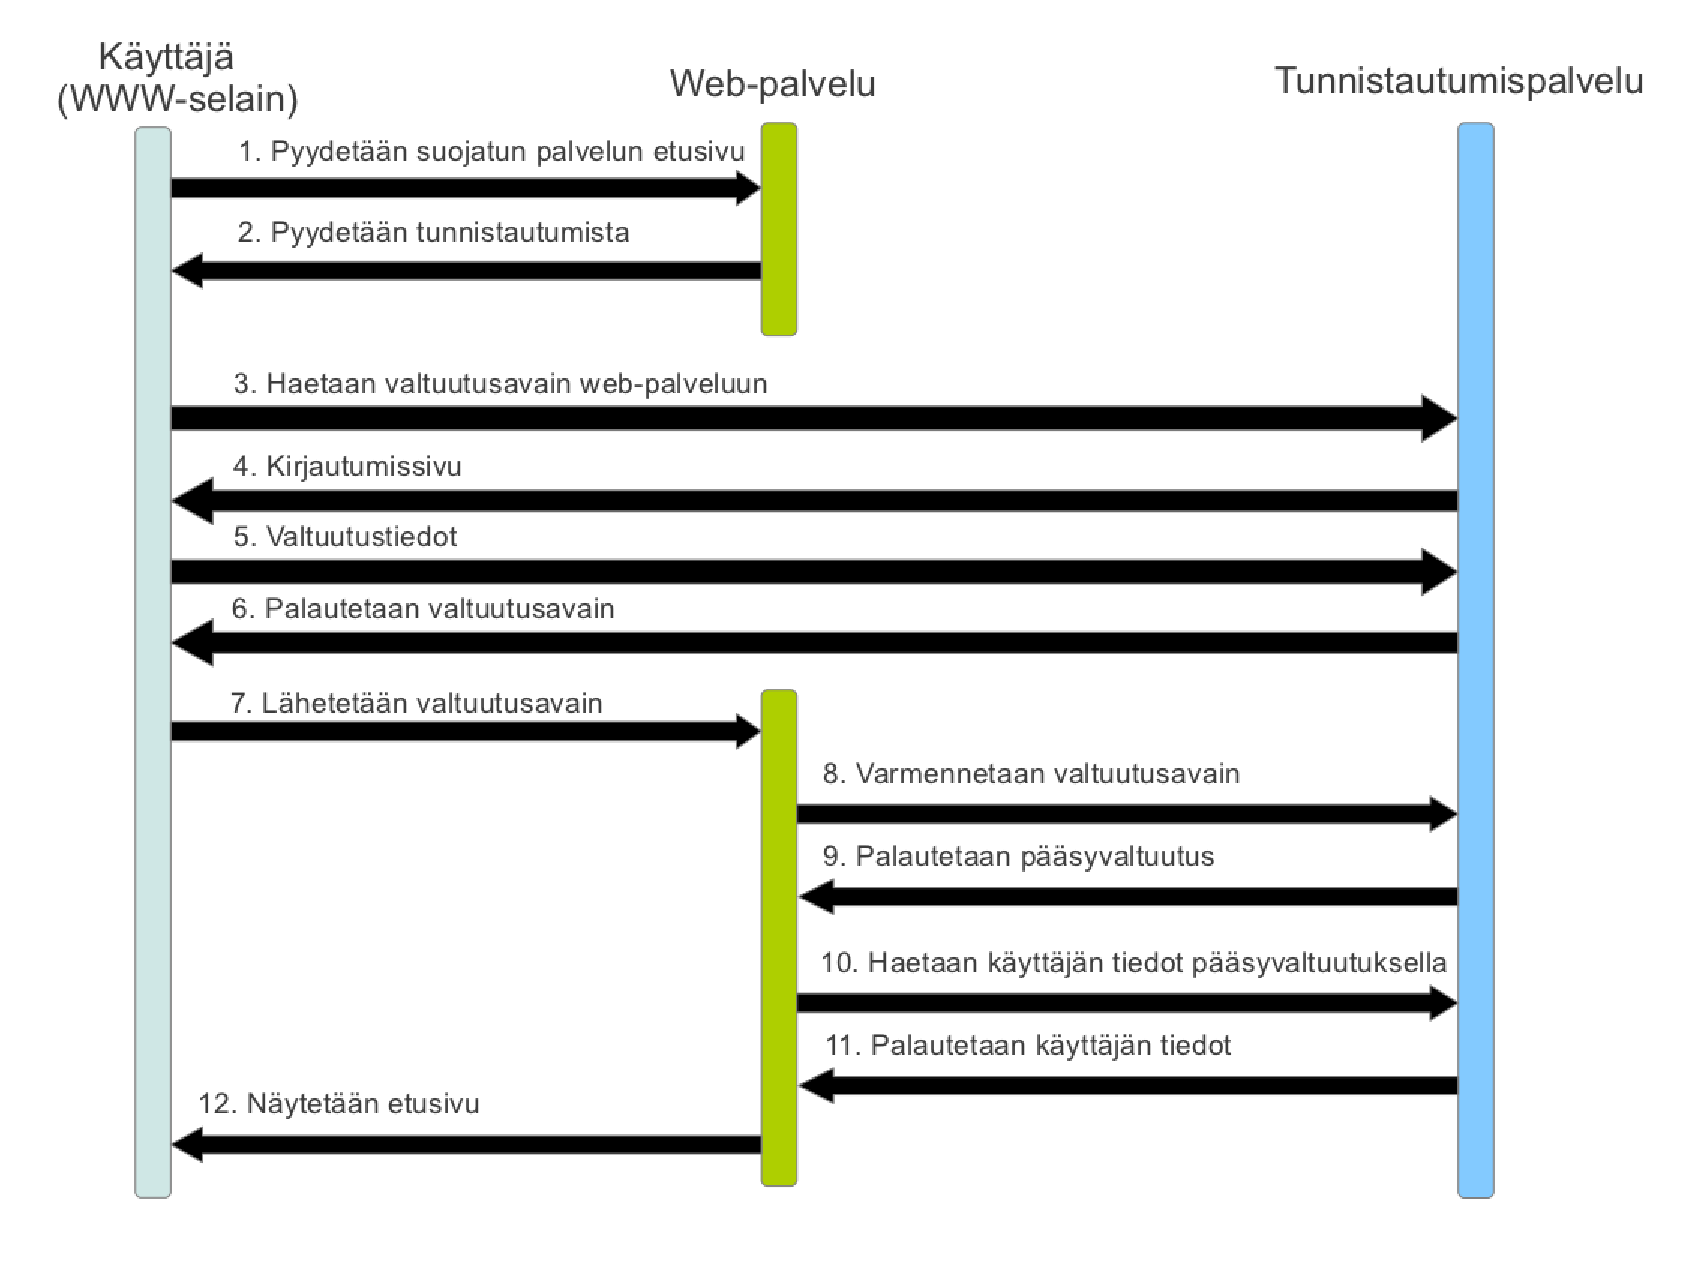
\includegraphics[width=\textwidth]{teknologiat/protokollat/oauth.eps}
\caption{OAuth sekvenssikaavio}%
\label{oauth}
\end{figure}

\section{Toteutus}
\section{Toteutuksen evaluaatio}
\section{Yhteenveto}
\bibliographystyle{tktl}
\bibliography{munBibTeXtiedosto}
\lastpage
\appendices
\internalappendix{\theappendix}{Eka liite}
Liitetekstiä.
\internalappendix{2}{Toka liite}
Liitetekstiä. Ehkä kuviakin.
\externalappendix{\theappendix}{Ohjelmalistaus joka ei sisälly
\LaTeX-tiedostoon}
\end{document}
